\begin{quote}
This is part 13 of Categories for Programmers. Previously:
\href{https://bartoszmilewski.com/2015/04/15/limits-and-colimits/}{Limits
and Colimits}. See the
\href{https://bartoszmilewski.com/2014/10/28/category-theory-for-programmers-the-preface/}{Table
of Contents}.
\end{quote}

Monoids are an important concept in both category theory and in
programming. Categories correspond to strongly typed languages, monoids
to untyped languages. That's because in a monoid you can compose any two
arrows, just as in an untyped language you can compose any two functions
(of course, you may end up with a runtime error when you execute your
program).

We've seen that a monoid may be described as a category with a single
object, where all logic is encoded in the rules of morphism composition.
This categorical model is fully equivalent to the more traditional
set-theoretical definition of a monoid, where we ``multiply'' two
elements of a set to get a third element. This process of
``multiplication'' can be further dissected into first forming a pair of
elements and then identifying this pair with an existing element ---
their ``product.''

What happens when we forgo the second part of multiplication --- the
identification of pairs with existing elements? We can, for instance,
start with an arbitrary set, form all possible pairs of elements, and
call them new elements. Then we'll pair these new elements with all
possible elements, and so on. This is a chain reaction --- we'll keep
adding new elements forever. The result, an infinite set, will be
\emph{almost} a monoid. But a monoid also needs a unit element and the
law of associativity. No problem, we can add a special unit element and
identify some of the pairs --- just enough to support the unit and
associativity laws.

Let's see how this works in a simple example. Let's start with a set of
two elements, \texttt{\{a,\ b\}}. We'll call them the generators of the
free monoid. First, we'll add a special element \texttt{e} to serve as
the unit. Next we'll add all the pairs of elements and call them
``products''. The product of \texttt{a} and \texttt{b} will be the pair
\texttt{(a,\ b)}. The product of \texttt{b} and \texttt{a} will be the
pair \texttt{(b,\ a)}, the product of \texttt{a} with \texttt{a} will be
\texttt{(a,\ a)}, the product of \texttt{b} with \texttt{b} will be
\texttt{(b,\ b)}. We can also form pairs with \texttt{e}, like
\texttt{(a,\ e)}, \texttt{(e,\ b)}, etc., but we'll identify them with
\texttt{a}, \texttt{b}, etc. So in this round we'll only add
\texttt{(a,\ a)}, \texttt{(a,\ b)} and \texttt{(b,\ a)} and
\texttt{(b,\ b)}, and end up with the set
\texttt{\{e,\ a,\ b,\ (a,\ a),\ (a,\ b),\ (b,\ a),\ (b,\ b)\}}.

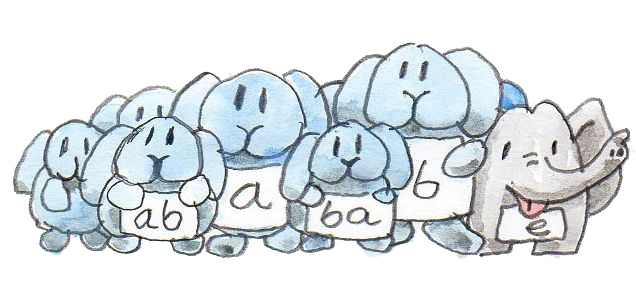
\includegraphics[width=4.54167in]{images/bunnies.jpg}

In the next round we'll keep adding elements like:
\texttt{(a,\ (a,\ b))}, \texttt{((a,\ b),\ a)}, etc. At this point we'll
have to make sure that associativity holds, so we'll identify
\texttt{(a,\ (b,\ a))} with \texttt{((a,\ b),\ a)}, etc. In other words,
we won't be needing internal parentheses.

You can guess what the final result of this process will be: we'll
create all possible lists of \texttt{a}s and \texttt{b}s. In fact, if we
represent \texttt{e} as an empty list, we can see that our
``multiplication'' is nothing but list concatenation.

This kind of construction, in which you keep generating all possible
combinations of elements, and perform the minimum number of
identifications --- just enough to uphold the laws --- is called a free
construction. What we have just done is to construct a \emph{free
monoid} from the set of generators \texttt{\{a,\ b\}}.

\subsection{Free Monoid in Haskell}\label{free-monoid-in-haskell}

A two-element set in Haskell is equivalent to the type \texttt{Bool},
and the free monoid generated by this set is equivalent to the type
\texttt{{[}Bool{]}} (list of \texttt{Bool}). (I am deliberately ignoring
problems with infinite lists.)

A monoid in Haskell is defined by the type class:

\begin{verbatim}
class Monoid m where mempty :: m mappend :: m -> m -> m
\end{verbatim}

This just says that every \texttt{Monoid} must have a neutral element,
which is called \texttt{mempty}, and a binary function (multiplication)
called \texttt{mappend}. The unit and associativity laws cannot be
expressed in Haskell and must be verified by the programmer every time a
monoid is instantiated.

The fact that a list of any type forms a monoid is described by this
instance definition:

\begin{verbatim}
instance Monoid [a] where mempty = [] mappend = (++)
\end{verbatim}

It states that an empty list \texttt{{[}{]}} is the unit element, and
list concatenation \texttt{(++)} is the binary operation.

As we have seen, a list of type \texttt{a} corresponds to a free monoid
with the set \texttt{a} serving as generators. The set of natural
numbers with multiplication is not a free monoid, because we identify
lots of products. Compare for instance:

\begin{verbatim}
2 * 3 = 6 [2] ++ [3] = [2, 3] // not the same as [6]
\end{verbatim}

That was easy, but the question is, can we perform this free
construction in category theory, where we are not allowed to look inside
objects? We'll use our workhorse: the universal construction.

The second interesting question is, can any monoid be obtained from some
free monoid by identifying more than the minimum number of elements
required by the laws? I'll show you that this follows directly from the
universal construction.

\subsection{Free Monoid Universal
Construction}\label{free-monoid-universal-construction}

If you recall our previous experiences with universal constructions, you
might notice that it's not so much about constructing something as about
selecting an object that best fits a given pattern. So if we want to use
the universal construction to ``construct'' a free monoid, we have to
consider a whole bunch of monoids from which to pick one. We need a
whole category of monoids to chose from. But do monoids form a category?

Let's first look at monoids as sets equipped with additional structure
defined by unit and multiplication. We'll pick as morphisms those
functions that preserve the monoidal structure. Such
structure-preserving functions are called \emph{homomorphisms}. A monoid
homomorphism must map the product of two elements to the product of the
mapping of the two elements:

\begin{verbatim}
h (a * b) = h a * h b
\end{verbatim}

and it must map unit to unit.\\
For instance, consider a homomorphism from lists of integers to
integers. If we map \texttt{{[}2{]}} to 2 and \texttt{{[}3{]}} to 3, we
have to map \texttt{{[}2,\ 3{]}} to 6, because concatenation

\begin{verbatim}
[2] ++ [3] = [2, 3]
\end{verbatim}

becomes multiplication

\begin{verbatim}
2 * 3 = 6
\end{verbatim}

Now let's forget about the internal structure of individual monoids, and
only look at them as objects with corresponding morphisms. You get a
category \textbf{Mon} of monoids.

Okay, maybe before we forget about internal structure, let us notice an
important property. Every object of \textbf{Mon} can be trivially mapped
to a set. It's just the set of its elements. This set is called the
\emph{underlying} set. In fact, not only can we map objects of
\textbf{Mon} to sets, but we can also map morphisms of \textbf{Mon}
(homomorphisms) to functions. Again, this seems sort of trivial, but it
will become useful soon. This mapping of objects and morphisms from
\textbf{Mon} to \textbf{Set} is in fact a functor. Since this functor
``forgets'' the monoidal structure --- once we are inside a plain set,
we no longer distinguish the unit element or care about multiplication
--- it's called a \emph{forgetful functor}. Forgetful functors come up
regularly in category theory.

We now have two different views of \textbf{Mon}. We can treat it just
like any other category with objects and morphisms. In that view, we
don't see the internal structure of monoids. All we can say about a
particular object in \textbf{Mon} is that it connects to itself and to
other objects through morphisms. The ``multiplication'' table of
morphisms --- the composition rules --- are derived from the other view:
monoids-as-sets. By going to category theory we haven't lost this view
completely --- we can still access it through our forgetful functor.

To apply the universal construction, we need to define a special
property that would let us search through the category of monoids and
pick the best candidate for a free monoid. But a free monoid is defined
by its generators. Different choices of generators produce different
free monoids (a list of \texttt{Bool} is not the same as a list of
\texttt{Int}). Our construction must start with a set of generators. So
we're back to sets!

That's where the forgetful functor comes into play. We can use it to
X-ray our monoids. We can identify the generators in the X-ray images of
those blobs. Here's how it works:

We start with a set of generators, \texttt{x}. That's a set in
\textbf{Set}.

The pattern we are going to match consists of a monoid \texttt{m} --- an
object of \textbf{Mon} --- and a function \texttt{p} in \textbf{Set}:

\begin{verbatim}
p :: x -> U m
\end{verbatim}

where \texttt{U} is our forgetful functor from \textbf{Mon} to
\textbf{Set}. This is a weird heterogeneous pattern --- half in
\textbf{Mon} and half in \textbf{Set}.

The idea is that the function \texttt{p} will identify the set of
generators inside the X-ray image of \texttt{m}. It doesn't matter that
functions may be lousy at identifying points inside sets (they may
collapse them). It will all be sorted out by the universal construction,
which will pick the best representative of this pattern.

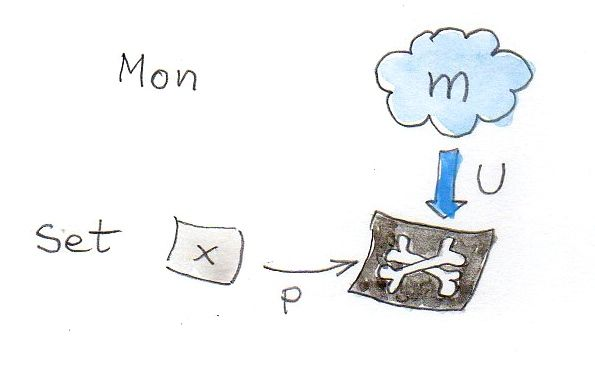
\includegraphics[width=3.12500in]{images/monoid-pattern.jpg}

We also have to define the ranking among candidates. Suppose we have
another candidate: a monoid \texttt{n} and a function that identifies
the generators in its X-ray image:

\begin{verbatim}
q :: x -> U n
\end{verbatim}

We'll say that \texttt{m} is better than \texttt{n} if there is a
morphism of monoids (that's a structure-preserving homomorphism):

\begin{verbatim}
h :: m -> n
\end{verbatim}

whose image under \texttt{U} (remember, \texttt{U} is a functor, so it
maps morphisms to functions) factorizes through \texttt{p}:

\begin{verbatim}
q = U h . p
\end{verbatim}

If you think of \texttt{p} as selecting the generators in \texttt{m};
and \texttt{q} as selecting ``the same'' generators in \texttt{n}; then
you can think of \texttt{h} as mapping these generators between the two
monoids. Remember that \texttt{h}, by definition, preserves the monoidal
structure. It means that a product of two generators in one monoid will
be mapped to a product of the corresponding two generators in the second
monoid, and so on.

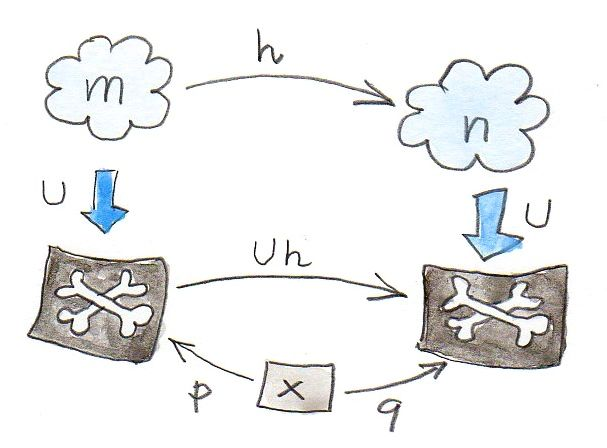
\includegraphics[width=3.12500in]{images/monoid-ranking.jpg}

This ranking may be used to find the best candidate --- the free monoid.
Here's the definition:

We'll say that \texttt{m} (together with the function \texttt{p}) is the
\textbf{free monoid} with the generators \texttt{x} if and only if there
is a \emph{unique} morphism \texttt{h} from \texttt{m} to any other
monoid \texttt{n} (together with the function \texttt{q}) that satisfies
the above factorization property.

Incidentally, this answers our second question. The function
\texttt{U\ h} is the one that has the power to collapse multiple
elements of \texttt{U\ m} to a single element of \texttt{U\ n}. This
collapse corresponds to identifying some elements of the free monoid.
Therefore any monoid with generators \texttt{x} can be obtained from the
free monoid based on \texttt{x} by identifying some of the elements. The
free monoid is the one where only the bare minimum of identifications
have been made.

We'll come back to free monoids when we talk about adjunctions.

\subsection{Challenges}\label{challenges}

\begin{enumerate}
\item
  You might think (as I did, originally) that the requirement that a
  homomorphism of monoids preserve the unit is redundant. After all, we
  know that for all \texttt{a}

\begin{verbatim}
h a * h e = h (a * e) = h a
\end{verbatim}

  So \texttt{h\ e} acts like a right unit (and, by analogy, as a left
  unit). The problem is that \texttt{h\ a}, for all \texttt{a} might
  only cover a sub-monoid of the target monoid. There may be a ``true''
  unit outside of the image of \texttt{h}. Show that an isomorphism
  between monoids that preserves multiplication must automatically
  preserve unit.
\item
  Consider a monoid homomorphism from lists of integers with
  concatenation to integers with multiplication. What is the image of
  the empty list \texttt{{[}{]}}? Assume that all singleton lists are
  mapped to the integers they contain, that is \texttt{{[}3{]}} is
  mapped to 3, etc. What's the image of \texttt{{[}1,\ 2,\ 3,\ 4{]}}?
  How many different lists map to the integer 12? Is there any other
  homomorphism between the two monoids?
\item
  What is the free monoid generated by a one-element set? Can you see
  what it's isomorphic to?
\end{enumerate}

Next:
\href{https://bartoszmilewski.com/2015/07/29/representable-functors/}{Representable
Functors}.

\subsection{Acknowledgments}\label{acknowledgments}

I'd like to thank Gershom Bazerman for checking my math and logic, and
André van Meulebrouck, who has been volunteering his editing help
throughout this series of posts.\\
\href{https://twitter.com/BartoszMilewski}{Follow @BartoszMilewski}

{43.193044} {11.286147}
